% Source: https://tex.stackexchange.com/a/659874/6880

\documentclass{article}

\usepackage{tikz}
\usetikzlibrary{matrix}
\tikzset{wordlematrix/.style={matrix of nodes, nodes={anchor=center, fill=bad, minimum height=1cm, minimum width=1cm}, column sep=2pt, row sep=2pt, color=white, font=\sffamily\Large\bfseries},
    g/.style={fill=great}, h/.style={fill=good},  n/.style={fill=none, color=black, draw=dark-border, thick,minimum size=1cm-\pgflinewidth}, e/.style={fill=none, color=black, draw=light-border, thick,minimum size=1cm-\pgflinewidth}}

\definecolor{great}{rgb}{0.416, 0.667, 0.392}
\definecolor{good}{rgb}{0.788, 0.706, 0.345}
\definecolor{bad}{rgb}{0.471, 0.486, 0.494}
\definecolor{light-border}{rgb}{0.827, 0.839, 0.855}
\definecolor{dark-border}{rgb}{0.529, 0.541, 0.549}
\definecolor{none}{rgb}{1,1,1}

\title{Here is a 
    
\begin{tikzpicture}[baseline=-1.5mm]
    \matrix(titlewordle)[wordlematrix, ampersand replacement=\&]{ 
    W \& |[g]|O \& |[g]|R \& D \& |[h]|L \& E\\
    };
    \end{tikzpicture}
    in a title}
\author{Sandy G}

\begin{document}
\maketitle

Here is a wordle in the document:
\[
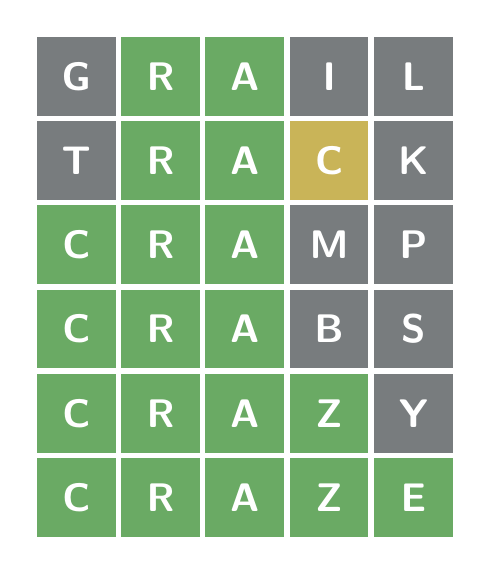
\begin{tikzpicture}
\matrix(example)[wordlematrix]{ 
G & |[g]|R & |[g]|A & I & L\\
T & |[g]|R & |[g]|A & |[h]|C & K\\
|[g]|C & |[g]|R & |[g]|A & M & P\\
|[g]|C & |[g]|R & |[g]|A & B & S\\
|[g]|C & |[g]|R & |[g]|A & |[g]|Z & Y\\
|[g]|C & |[g]|R & |[g]|A & |[g]|Z & |[g]|E\\
};
\end{tikzpicture}
\]
Here is a wordle to complete:
\[
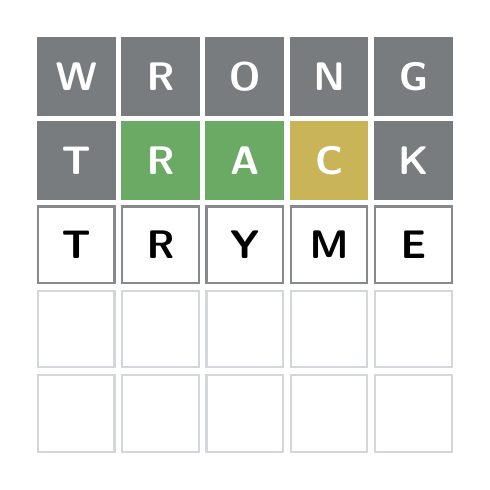
\begin{tikzpicture}
\matrix(example)[wordlematrix]{ 
W & R & O & N & G\\
T & |[g]|R & |[g]|A & |[h]|C & K\\
|[n]|T&|[n]|R&|[n]|Y&|[n]|M&|[n]|E\\
|[e]|& |[e]| & |[e]|& |[e]| & |[e]|\\
|[e]|& |[e]| & |[e]|& |[e]| & |[e]|\\
};
\end{tikzpicture}
\]
I did it!

\end{document}